\mbox{$\displaystyle -\,\frac{1}{6}$\,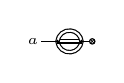
\begin{tikzpicture}[x=0.340cm, y=0.340cm, line width=0.420pt, baseline={([yshift=-0.6ex]0,0)}]
  \draw[double, double distance=0.781pt] (0.000,0.000) arc[start angle=186.026, end angle=353.974, radius=0.452];
  \draw[double, double distance=0.781pt] (0.000,0.000) -- (0.900,0.000);
  \draw[double, double distance=0.781pt] (0.000,0.000) arc[start angle=173.974, end angle=6.026, radius=0.452];
  \draw (0.000,0.000) -- (-0.600,0.000);
  \draw (0.900,0.000) -- (1.300,0.000);
  \draw[fill=white] (1.300,0.000) circle (0.100);
  \draw[line width=0.298pt] (1.370,0.070) -- (1.230,-0.070) (1.370,-0.070) -- (1.230,0.070);
  \fill (0.000,0.000) circle (0.064);
  \fill (0.900,0.000) circle (0.064);
  \node[font=\tiny, inner sep=0pt, anchor=0] at (-0.690,0.000) {$a$};
\end{tikzpicture}}
\diagramgap
\mbox{$\displaystyle -\,\frac{1}{4}$\,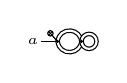
\begin{tikzpicture}[x=0.340cm, y=0.340cm, line width=0.420pt, baseline={([yshift=-0.6ex]0,0)}]
  \draw[double, double distance=0.781pt] (0.000,0.000) arc[start angle=186.026, end angle=353.974, radius=0.452];
  \draw[double, double distance=0.781pt] (0.000,0.000) arc[start angle=173.974, end angle=6.026, radius=0.452];
  \draw[double, double distance=0.781pt] (0.900,0.000) arc[start angle=180.000, end angle=540.000, radius=0.280];
  \draw (0.000,0.000) -- (-0.600,0.000);
  \draw (0.000,0.000) -- (-0.263,0.301);
  \draw[fill=white] (-0.263,0.301) circle (0.100);
  \draw[line width=0.298pt] (-0.193,0.371) -- (-0.333,0.231) (-0.193,0.231) -- (-0.333,0.371);
  \fill (0.000,0.000) circle (0.064);
  \fill (0.900,0.000) circle (0.064);
  \node[font=\tiny, inner sep=0pt, anchor=0] at (-0.690,0.000) {$a$};
\end{tikzpicture}}
